%  Typ dokumentu - článek, prezentace aj.
\documentclass[english]{article}

%  Nastaví vstupní a výstupní kódování znaků (encoding) a lokalizace
\usepackage[T1]{fontenc}
\usepackage[utf8]{inputenc}
\usepackage[english,czech]{babel}
\usepackage{icomma}
\usepackage{lmodern}

%  Formát papíru a odsazení od jeho okrajů
\usepackage[letterpaper]{geometry}
\geometry{verbose,tmargin=1.5cm,bmargin=2cm,lmargin=2cm,rmargin=2cm}

%  Umožňuje pracovat s grafikou
\usepackage{graphicx}
\usepackage{bigstrut}

%  Automaticky odsadí i první paragraf v každé sekci
\usepackage{indentfirst}

%  Umožňuje rozdělovat obsah na více sloupců
\usepackage{multicol}
\usepackage{booktabs}

%  Umožňuje používat hypertextové odkazy, nastavuje jejich barvu a
%  vlastnosti
\usepackage[unicode]{hyperref}
\hypersetup{
colorlinks=true, citecolor=blue, filecolor=blue, linkcolor=blue,
urlcolor=blue
}

%  Umožnění odstranění italiky u jednotek
\newcommand{\unit}[1]{\mathrm{#1}}

%  Formátování stránek, empty = odstraní číslování
% \pagestyle{empty}

%  Řádkování
\linespread{1.2}

%  Lepší zobrazování matematiky (rozšíření sum o \limits atd.)
\everymath{\displaystyle}
\usepackage{amsmath, amsthm, amssymb}

% Umožní psát přes \mathbb{N/R/Q/..} množiny čísel
\usepackage{amssymb}

%  Velikost fontu matematických výrazů v dokumentu lze pro danou
% základního fontu dokumentu upravit pomocí:
% \DeclareMathSizes{X}{Y}{Z}{U} kde:
% X je velikost fontu v dokumentu, pro kterou se matematika upraví
% Y je standartní velikost fontu matematiky
% Z je velikost fontu zmenšených (vnořených výrazů)
% U je velikost fontu ještě více zmenšených (vnořených výrazů).
\DeclareMathSizes{10}{10.5}{9}{9}

%  Nastaví autora, název, datum, skupinu měření apod. (můj vlastní
% příkaz, umožní znovu-použití v dokumentu)
\newcommand{\Author}{David Roesel}
\newcommand{\Coauthor}{Tereza Schönfeldová}
\newcommand{\Institute}{FJFI ČVUT v Praze}
\newcommand{\Subject}{FYZIKÁLNÍ PRAKTIKUM I}
\newcommand{\Group}{7}
\newcommand{\Circle}{ZS 5}
\newcommand{\Title}{Úloha \#4  \\Poissonova konstanta a měření dutých objemů}
\newcommand{\Date}{6.12.2013}

% Začátek dokumentu - Formátování na výstup
\begin{document}

% Interní proměnné, možno zobrazovat u prezentací, používají se při
% generování pomocí \titlepage apod.
\author{\Author}
\title{\Title}
\date{\Date}

%  Lokalizace některých názvů do češtiny
\renewcommand{\figurename}{Obr.}
\renewcommand{\tablename}{Tab.}
\renewcommand{\refname}{Reference}

% --- Hlavička dokumentu -----------------------------------------------

\setlength{\parindent}{0cm}
\begin{multicols}{2}
\textbf{\Subject \\
        \Institute \\[0.1cm]
%\large  \Title \\[0.5cm]
\Title \\[0.5cm]
}
\begin{tabular}{rlrl}
\large Datum měření: & \Date & \large Skupina: & \Group \\
\large Jméno: & \Author & \large Kroužek:  & \Circle\\
\large Spolupracovala: & \Coauthor &\large Klasifikace:\\
\end{tabular}

\begin{flushright}

\includegraphics[scale=0.28]{../../_meta/fjfi_standart.pdf}
\hspace{0.2cm}
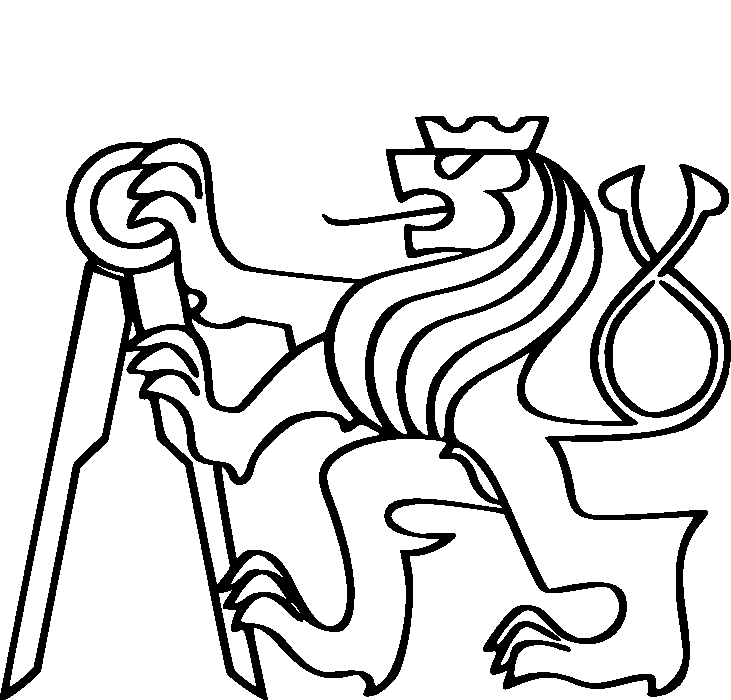
\includegraphics[scale=0.28]{../../_meta/cvut_standart.pdf}
\end{flushright}
\end{multicols}
\hrule
\vspace{0.5cm}

% ----------------------------------------------------------------------


% --- Tělo dokumentu ---------------------------------------------------
\setlength{\parindent}{0.5cm}
\section{Pracovní úkoly}

	\subsection{Měření dutých objemů vážením a kompresí plynu}
		\begin{enumerate}
			\item Jednolitrovou láhev zvažte prázdnou.
			\item Jednolitrovou láhev zvažte plnou vody.
			\item Z obou výsledků určete objem lahve.
			\item Objem prázdné jednolitrové lahve určete kompresí plynu.
			\item Stejným postupem změřte objem hadičky spojující byretu s měřeným prostorem. Tuto hodnotu odečtěte od výsledku podle bodu 4.
		\end{enumerate}
		
	\subsection{Měření Poissonovy konstanty vzduchu}
			\begin{enumerate}
			\item Změřte kompresí plynu objem baňky systému s kmitajícím pístkem.
			\item Změřte Poissonovu konstantu metodou adiabatické expanze a současně metodou kmitajícího pístku.
			\item Oba výsledky porovnejte. Výsledek metody kmitajícího pístku považujte za tabulkovou hodnotu Poissonovy konstanty.
		\end{enumerate}	
	
\section{Vypracování}

	\subsection{Použité přístroje}
	
		\subsubsection{Měření dutých objemů vážením a kompresí plynu}
			Měřený objem (láhev s kohoutem), speciální plynová byreta s porovnávacím ramenem, katetometr, váhy, teploměr, voda.
		
		\subsubsection{Měření Poissonovy konstanty vzduchu}
			Teploměr, skleněná báň se dvěma kohouty, otevřený manometr, gumový měch, stopky s optickou branou, systém s pumpou a kmitajícím pístkem.
						
	\subsection{Teoretický úvod}
			
			\subsubsection{Měření objemu vážením}
					Zajímá nás vnitřní objem nádoby, který zjistíme jeho vyplněním kapalinou o známé hustotě - v našem případě vodou. Nádobu následně zvážíme naplněnou a prázdnou a pro vnitřní objem bude platit následující vztah
					\begin{equation}\label{eq:objem_vazeni}
						V = \frac{m_v}{\rho_v}=m_v V_v,
					\end{equation}
					kde $m_v$ je hmotnost vody, $\rho_v$ její hustota a $V_v$ objem jednoho gramu vody. Ten získáme pomocí vztahu 
					\begin{equation}\label{eq:objem_V_v}
						V_v = 0,9998(1+0,00018t) \left[\frac{cm^3}{g},^\circ C\right],
					\end{equation}
					ve kterém je $t$ teplota vody.
				
			\subsubsection{Měření objemu kompresí plynu}
					V případě, že se nedá měřit objem vážením, můžeme volit metodu využívající plynu. Pomocí speciální aparatury sestavené podle Obr. \ref{fig:aparatura1} vyrovnáme hladiny vody v byretě a pomocné trubici (za působení atmosferického tlaku) a následně ramenu, které vede do měřeného objemu (byretou), zavřeme vnější ventil. Tím, že poté natlakujeme spodní nádrž s vodou, zvýšíme tlak na měřený objem a ten se zmenší z původní hodnoty $V_0$ na novou hodnotu $V_1$. Tlaky v kapalině se musí vyrovnávat, takže z rozdílu hladin v obou trubicích $\Delta h$ můžeme určit změnu tlaku uvnitř měřené nádoby $\Delta p$ v porovnání s původním (atmosferickým) tlakem $p$. Z Boyle-Mariottova zákona dostáváme vzorec 
					\begin{equation}\label{eq:objem_komprese}
						V = (V_0-V_1)\frac{p}{\Delta p},
					\end{equation}		 
					kde $\Delta p$ určíme ze vztahu 
					\begin{equation}\label{eq:objem_Delta_p}
						V =  \Delta h \rho_v g.
					\end{equation}		
					Ještě nedefinovanými veličinami jsou hustota vody $\rho_v$ a gravitační zrychlení $g$.
					 
			\subsubsection{Měření Poissonovy konstanty vzduchu Clémentovou-Désormesovou metodou}
					V následujících dvou měřeních je hlavním úkolem změření tzv. Poissonovy konstanty vzduchu, která je definována jako poměr měrných tepel při konstantním tlaku $C_p$ a konstantním objemu $C_v$, tedy jako
					\begin{equation}
						\varkappa = \frac{C_p}{C_v}.
					\end{equation}
					Jednou z nejjednodušších metod určení této konstanty je metoda Clémentova-Désormesova. V aparatuře k této metodě (viz Obr. \ref{fig:aparatura2}) je nádoba pod atmosferickým tlakem $b$ a je k ní připojen manometr s vodou. Tím, že balónkem zvýšíme tlak v nádobě z původních $b$ na novou hodnotu $p_1$, vytvoříme rozdíl hladin v manometru $\Delta h$. Krátkým stisknutím ventilku na nádobě následně umožníme plynu adiabaticky expandovat, čímž se zvýší objem z $V_1$ na $V_2$ a sníží se teplota. Tlak se tím zároveň opět vrátí na původní hodnotu $b$, ale při následném izochorickém oteplování vzroste na $p_2$ a na manometru bude pozorovatelný jiný rozdíl hladin $\Delta h'$. Během tohoto izotermického děje platí 
					\begin{equation}\label{eq:izoterma}
						\frac{p_1}{p_2} = \frac{V_2}{V_1}
					\end{equation}		
					a (za předpokladu, že je vzduch ideálním plynem) pro adiabatický děj také
					\begin{equation}
						\frac{p_1}{b} = \left( \frac{V_1}{V_2}\right)^\varkappa.
					\end{equation}
					Za předpokladu, že je $h$ mnohem menší než $b$, můžeme po dosazení těchto rovnic do sebe použít rozvoj pro logaritmus a odvodit finální vzorec
					\begin{equation}\label{eq:psst}
						\varkappa = \frac{\Delta h}{\Delta h-\Delta h'} .
					\end{equation}
					Tento výpočet by byl přesný v případě okamžité změny objemu při zmáčknutí pístu. Toho ale reálně nejde dosáhnout, a tak pro získání hodnoty v nule musíme lineárně extrapolovat do nuly závislost změřené Poissonovy konstanty $\varkappa$ na době $t$, po jakou byl píst otevřen. 
							
			\subsubsection{Měření Poissonovy konstanty vzduchu metodou kmitajícího pístku}
					Poissonovu konstantu můžeme ještě přesněji změřit pomocí metody kmitajícího pístku. Máme-li nádobu, do které přivádíme plyn a na kterou je ze shora namontována trubice s pístkem a bočním otvorem (tak jako na Obr. \ref{fig:aparatura3}), můžeme zvýšením tlaku v nádobě donutit pístek ke stoupání. Jakmile se dostane nad otvor, bude otvorem plyn unikat a tlak v soustavě opět klesne, čímž bude pístku umožněno klesnout zpět pod otvor. Vhodným nastavením aparatury můžeme donutit pístek ke kmitání kolem otvoru a pomocí senzoru měřit periodu jeho kmitů. Pro Poissonovu konstantu potom bude platit
					\begin{equation}\label{eq:pistek}
							\varkappa = \frac{4mV}{T^2pr^4}, \qquad p=b+\frac{mg}{\pi r^2},
					\end{equation}
					kde $m$ je hmotnost pístku, $V$ objem nádoby, $T$ perioda kmitů, $p$ tlak v nádobě, $b$ je atmosferický tlak, $r$ poloměr pístku a $g$ tíhové zrychlení.
					
	\subsection{Postup měření}
			\subsubsection{Měření objemu vážením}
				   Před začátkem celého měření jsme z teploměru odečetli teplotu v praktiku. Z měřené láhve jsme nejdříve vylili vodu, která v ní byla, a pokusili se ji osušit. Následně jsme ji třikrát zvážili (i s víčkem) a zaznamenali hodnoty. Po měření objemu kompresí plynu (viz další měření) jsme pak lahev naplnili vodou z kohoutku a to až po vrchní okraj víčka. Lahev jsme následně znovu třikrát zvážili. 
					
			\subsubsection{Měření objemu kompresí plynu}
					Aparatura k tomuto pokusu již byla sestavena (viz Obr. \ref{fig:aparatura1}). K byretě jsme pomocí hadice připojili lahev z minulého měření a měřili podle následujícího postupu:
					\begin{enumerate}
							\item Se zavřeným ventilem 5 na tlakovači a otevřeným horním ventilem 6 vyrovnáme pomocí balónku hladiny v tubici a byretě.
							\item Zaznamenáme si objem $V_0$ a nastavíme katetometr na předpokládanou výšku hladiny v trubici.
							\item Uzavřeme ventil 6 a zvyšujeme pomocí balónku tlak v soustavě tak, aby se objem změnil z $V_0$ na $V_1$. 
							\item Katetometrem odečteme co nejrychleji po sobě hodnoty výšky hladiny $h_1$ a $h_2$ v trubici a byretě.
							\item Z byrety odečteme nový objem $V_1$ a otevřením ventilu 5 snížíme tlak i hladiny v obou trubicích.
							\item Předchozí kroky opakujeme desetkrát pro láhev a desetkrát pro lahvičku s uzavřeným hrdlem.
					\end{enumerate}
					 
			\subsubsection{Měření Poissonovy konstanty vzduchu Clémentovou-Désormesovou metodou}
					Aparatura již byla sestavena v podobě nádoby se dvěma ventily a připojeným manometrem (viz Obr. \ref{fig:aparatura2}). Při vlastním měření jsme postupovali následovně:
					\begin{enumerate}
							\item Se zavřeným ventilem $K$ a s otevřeným $K'$ zvýšíme pomocí balónku tlak v nádobě. 
							\item Uzavřeme první ventil, necháme chvíli ustálit hladiny v manometru a odečteme jejich hodnoty.
							\item Krátce otevřeme ventil $K$ a necháme plyn adiabaticky expandovat.
							\item Zaznamenáme dobu otevření ventilu z optického senzoru.
							\item Se zavřenými ventily opět necháme ustálit hladiny v manometru a odečteme jejich hodnoty.
							\item Předchozí kroky opakujeme, dokud nezískáme deset měření.
					\end{enumerate}
							
			\subsubsection{Měření Poissonovy konstanty vzduchu metodou kmitajícího pístku}
					Aparatura již byla sestavena (viz Obr. \ref{fig:aparatura3}), zbývalo jen zapnout čítač kmitů a pumpu, která zvyšovala tlak v nádobě. Zvyšování tlaku jsme upravili tak, aby pístek kmital kolem otvoru v trubici a více než desetkrát jsme změřili, kolikrát kmitne za dobu pěti minut. Z dokumentů na místě jsme zjistili konstanty potřebné k výpočtu, včetně objemu nádoby z tohoto úkolu, který jsme tím pádem neměřili. Toto měření jsme prováděli během všech ostatních, jelikož nevyžadovalo stálou pozornost. Dávali jsme si také pozor, aby amplituda pístku neklesla pod senzor a nepřišli jsme tak o nějaké kmity.
					
	\begin{figure}[h!]
	\centering
	\begin{minipage}{.40\textwidth}
	  \centering
					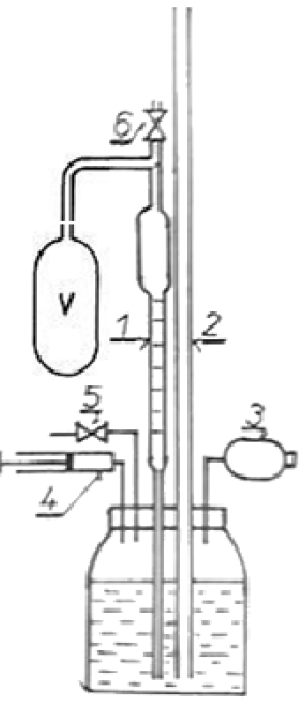
\includegraphics[width=5cm]{att/aparatura1.png}
					\vspace*{-0.5cm}
					\caption{Schéma aparatury pro měření objemů kompresí plynů (1-byreta, 2-trubice, 3-balónek, 5-ventil na tlakovači a 6-ventil na byretě). \cite{bib:repo}}
					\label{fig:aparatura1}
	\end{minipage}%
	\hfill
	\begin{minipage}{.55\textwidth}
			\begin{minipage}{.90\textwidth}
			  \centering
							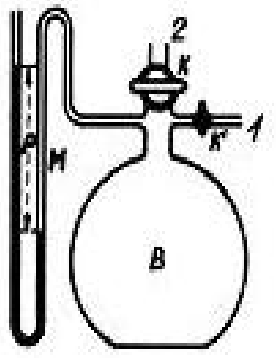
\includegraphics[width=2cm]{att/aparatura2.png}
							
							\caption{Schéma Clémentova-Désormesova přístroje pro určení $\varkappa$ .\cite{bib:zadani2}}
							\label{fig:aparatura2}
							\vspace*{1cm}
			
			  \centering
							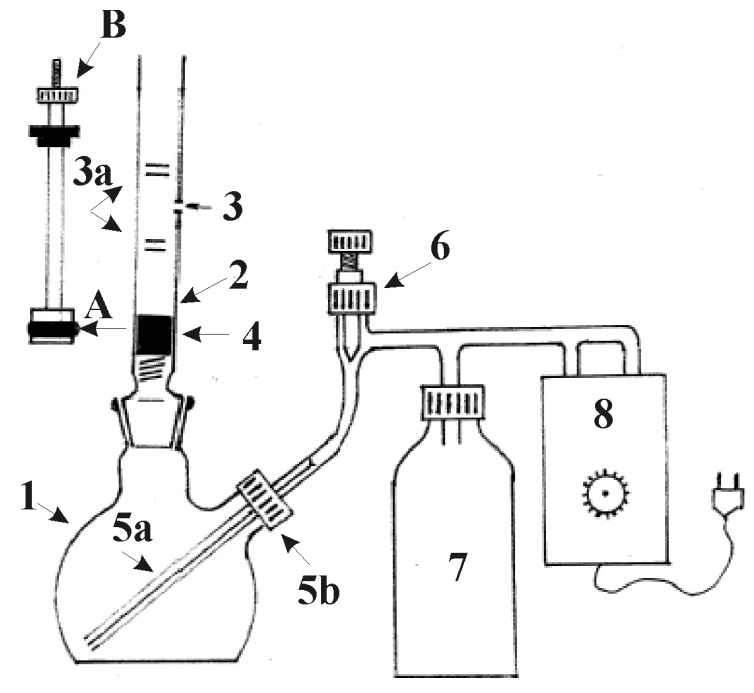
\includegraphics[width=7cm]{att/aparatura3.png}
							\caption{Schéma aparatury pro měření $\varkappa$ metodou kmitajícího pístku (1-nádoba, 3-otvor, 4-pístek, 8-pumpa).  \cite{bib:zadani3}}
							\label{fig:aparatura3}
			\end{minipage}
	\end{minipage}
	\end{figure}					
	\subsection{Naměřené hodnoty}
			\subsubsection{Měření objemu vážením}
				   Naměřené hodnoty hmotností jsou v Tab. \ref{tab:hmotnosti}. Hmotnost prázdné lahve (s našroubovaným víčkem) jsme určili jako $m_1 = (573,24 \pm 0,01)$ g, hmotnost plné lahve pak jako $m_2 = (1564 \pm 1)$ g. Z teploměru v praktiku jsme během měření odečetli hodnotu $t = (23,0\pm0,5) \unit{\ ^\circ C}$ s chybou poloviny nejmenšího dílku. Z teploty jsme určili pomocí (\ref{eq:objem_V_v}) i s chybou (\ref{eq:chyba_neprime_mereni}) objem jednoho gramu vody jako  $V_v = (1,0039\pm0,0001)\unit{\ cm^3}$ a z toho pak  pomocí (\ref{eq:objem_vazeni}) i s chybou (\ref{eq:chyba_neprime_mereni}) celkový objem lahve jako 
				   \begin{equation}
				   		V_{vazeni} = (995\pm1)\unit{\ cm^3}.
				   \end{equation}

% Table generated by Excel2LaTeX from sheet 'List1'
\begin{table}[htbp]
\catcode`\-=12 % HAX na enable cline v českym bable
  \centering
  
    \begin{tabular}{|r|r|r|r|r|}
\cline{2-5}    \multicolumn{1}{r|}{} & $m_1$ [g] & $\sigma_{m_1}$ [g] & $m_2$ [g] & $\sigma_{m_2}$ [g] \bigstrut\\
\cline{2-5}    \multicolumn{1}{r|}{} & 573,26 & 0,02  & 1564  & 1 \bigstrut\\
\cline{2-5}    \multicolumn{1}{r|}{} & 573,24 & 0,02  & 1564  & 1 \bigstrut\\
\cline{2-5}    \multicolumn{1}{r|}{} & 573,24 & 0,02  & 1564  & 1 \bigstrut\\
    \hline
    $\overline{m}\pm \sigma_{m}$ & 573,25 & 0,01  & 1564  & 1 \bigstrut\\
    \hline
    \end{tabular}%

 \caption{Naměřené hodnoty pro měření objemu vážením: $m_1$, $\sigma_{m_1}$ je hmotnost prázdné láhve s chybou (\ref{eq:chyba_aritmetickeho_prumeru}),  $m_2$, $\sigma_{m_2}$ pak analogicky pro láhev naplněnou vodou.}
 \label{tab:hmotnosti}%
\end{table}%

	
					
			\subsubsection{Měření objemu kompresí plynu}
					Naměřené hodnoty pro měření objemu láhve s hadičkou a samotné hadičky jsou vyneseny v Tab. \ref{tab:komprese_1} a Tab. \ref{tab:komprese_2}. Z dokumentů u úlohy jsme si opsali hodnotu odpovídající jednomu dílku byrety jako $\Delta V =0,656\unit{\ cm^3}.$ Vzhledem k tomu, že byl barometr v praktiku rozbitý, jsme uvažovali atmosferický tlak (pro tuto i všechny další úlohy) jako $p_A = 1010$ hPa \cite{bib:tlak}. Hustotu vody jsme určili jako převrácenou hodnotu $V_v$ z předchozí úlohy se stejným způsobem odvozenou chybou $\rho = (0,99608\pm0,00009) \unit{\ g\cdot cm^3}$. Ze změřených hodnot $\Delta h$ jsme určili podle (\ref{eq:objem_Delta_p}) s chybou (\ref{eq:chyba_neprime_mereni}) změnu tlaku $\Delta p$ při každém měření a z ní poté vždy ze vztahu (\ref{eq:objem_komprese}) objem.  Váženým průměrem (\ref{eq:vazeny_prumer}) potom dostáváme finální hodnotu objemu láhve s hadičkou $V_{l+h}$ a objemu samotné hadičky $V_h$ jako
				   \begin{equation}
				   		V_{l+h} = (960,1\pm0,7)\unit{\ cm^3}, \qquad V_{h} = (26,3\pm0,3)\unit{\ cm^3}.
				   \end{equation}					 
				   Z toho poté odečtením dostáváme i s chybou (\ref{eq:chyba_neprime_mereni}) finální hodnotu objemu měřené láhve jako
				   \begin{equation}
				   		V_{komprese} = (933,8\pm0,7)\unit{\ cm^3}.
				   \end{equation}
					 
			\subsubsection{Měření Poissonovy konstanty vzduchu Clémentovou-Désormesovou metodou}
					Naměřené hodnoty jsou uvedeny v Tab. \ref{tab:poisson_clement}. Pro každé měření jsme počítali Poissonovu konstantu $\varkappa$ dle vzorce (\ref{eq:psst}) s chybou (\ref{eq:chyba_neprime_mereni}). Následně jsme tyto hodnoty vynesli do grafu na Obr. \ref{fig:graf} a lineárním proložením extrapolovali do nuly. Výslednou hodnotu a chybu Poissonovy konstanty jsme tím pádem určili z parametrů fitu jako
				   \begin{equation}
				   		\varkappa = (1,37\pm0,01).
				   \end{equation}
				   

							
			\subsubsection{Měření Poissonovy konstanty vzduchu metodou kmitajícího pístku}
					Naměřené hodnoty počtu kmitů a z nich vypočítaných period jsou vyneseny v Tab. \ref{tab:pistek}. Z aritmetického průměru period a z hodnot konstant uvedených v dokumentu u úlohy (Tab. \ref{tab:konstanty}) jsme následně podle (\ref{eq:pistek}) spočítali i s chybou (\ref{eq:chyba_neprime_mereni}) Poissonovu konstantu jako
					\begin{equation}
				   		\varkappa = (1,387\pm0,001).
				   \end{equation}

% Table generated by Excel2LaTeX from sheet 'List1'
\begin{table}[h!]
  \centering
    \begin{tabular}{rrrrrr}
    \toprule
    $b$ [hPa] & $m$ [kg] & $r$ [m] & $g \unit{\ [m/s^2]}$ & $V$ [l] & $p$ [hPa] \\
    \midrule
    1010  & 0,00459 & 0,00595 & 9,81  & 0,00113 & 1014,05 \\
    \bottomrule
    \end{tabular}%
 \caption{Konstanty nejen z dokumentů u úlohy: $m$ je hmotnost pístku, $V$ objem nádoby, $r$ poloměr pístku, $g$ tíhové zrychlení, $b$ námi používaný atmosferický tlak a $p$ z toho spočítaný tlak v nádobě.}
   \label{tab:konstanty}%
\end{table}%
				   
							
	\subsection{Diskuse}
			\subsubsection{Měření objemu vážením}
					Tato metoda určení objemu byla z námi vyzkoušených dvou přesnější  s hodnotou $V_{vazeni} = (995\pm1)\unit{\ cm^3}$. Chyby při měření mohly ale nastat tím, že láhev nebyla před vážením naprázdno zcela suchá, jelikož jsme z ní museli vylévat vodu. Při druhém vážení (když byla láhev plná) se nám zase nepodařilo dostat z objemu všechny bublinky vzduchu a láhev nebyla zcela suchá na povrchu. Žádný z těchto jevů by však neměl hodnotu ovlivnit příliš.
					
			\subsubsection{Měření objemu kompresí plynu}
					Tato metoda nám sice dala hodnotu s menší statistickou chybou $V_{komprese} = (933,8\pm0,7)\unit{\ cm^3}$ než metoda předchozí, není ale pochyb, že byla značně ovlivněna systematickými chybami. Při odečítání výšky hladin jsme si sice velmi dobře procvičili používání katetometru, ale vzhledem k tomu, jak dlouho trvá přesun pohledu z hladiny v trubici na hladinu v byretě, se dá říci, že téměř nemá smysl určovat jejich výšky s takovou přesností. Měření by se dalo zlepšit použitím dvou katetometrů a sledováním obou hladin najednou, lepším utěsněním systému, aby hladiny neklesaly tak rychle, a nakonec měřením objemu na přesnějším měřítku. Řádově ale hodnota odpovídá odhadu a měření můžeme prohlásit za úspěšné.
					
			\subsubsection{Měření Poissonovy konstanty vzduchu Clémentovou-Désormesovou metodou}
					Touto metodou jsme se dobrali k výsledku $\varkappa = (1,37\pm0,01)$, který jsme finálně získali lineární extrapolací naměřené závislosti a jeho hodnota je velmi podobná té z následujícího měření, kterou bereme jako tabulkovou. K největším nepřesnostem došlo u této metody při měření času, po který byl otevřen horní ventil. Opakovaně se nám totiž stalo, že jsme ho zmáčkli (aniž bychom zakrývali senzor) a i přesto, že bylo slyšet unikající vzduch a že se změnily hladiny v manometru, senzor ukazoval nulový čas. Měření by šlo zpřesnit použitím lepšího senzoru otevření ventilu. Netěsnost aparatury byla, například v porovnání s první úlohou, zanedbatelná.
			
			\subsubsection{Měření Poissonovy konstanty vzduchu metodou kmitajícího pístku}	
					Toto měření bylo z našich dvou metod přesnější a dalo nám hodnotu $\varkappa = (1,387\pm0,001)$. Po počátečních problémech s nestálostí amplitudy pístku se velikost jeho kyvů ustálila a měření probíhalo bez problémů. Patrný nebyl ani zdroj výrazných systematických chyb, k některým mohlo dojít velikostí použitých konstant.

\section{Závěr}
		Láhev jsme úspěšně zvážili prázdnou a plnou a určili jsme z toho objem lahve na $V_{vazeni} = (995\pm1)\unit{\ cm^3}$. Ten samý objem jsme změřili také kompresí plynu jako $V_{komprese} = (933,8\pm0,7)\unit{\ cm^3}$ a uvedli, proč se hodnoty liší. Objem baňky systému s kmitajícím pístkem jsme neměřili, jelikož byl uveden v dokumentech u úlohy. Poissonovu konstantu jsme následně změřili přesně metodou kmitajícího pístku jako $\varkappa = (1,387\pm0,001)$ a s menší přesností pak z oddiskutovaných důvodů Clémentovou-Désormesovou metodou a lineární extrapolací jako $\varkappa = (1,37\pm0,01)$. 
			
\section {Použitá literatura}
% --- Literatura a reference -------------------------------------------
\begingroup
\renewcommand{\section}[2]{}

\begin{thebibliography}{9}
\bibitem{bib:zadani1} Kolektiv KF, \emph{Návod k úloze: Měření dutých objemů vážením a kompresí plynu} [Online], [cit. \today] \newline 
http://praktikum.fjfi.cvut.cz/pluginfile.php/105/mod\_resource/content/3/4\_Dute\_objemy.pdf

\bibitem{bib:zadani2} Kolektiv KF, \emph{Návod k úloze: Určení Poissonoyy konstanty vzduchu} [Online], [cit. \today] \newline 
http://praktikum.fjfi.cvut.cz/pluginfile.php/106/mod\_resource/content/2/4\_Poissonova\_konstanta.pdf

\bibitem{bib:zadani3} Kolektiv KF, \emph{Návod k úloze: Měření Poissonovy konstanty kmitajícím pístkem} [Online], [cit. \today] \newline 
http://bit.ly/PRAuloha4pistek

%\bibitem{bib:h3} Petr Chaloupka, \emph{Jak zpracovávat data} [Online], [cit. \today] \newline  https://dl.dropboxusercontent.com/u/11296940/zfm/h3.pdf

%\bibitem{bib:navody} Kolektiv KF, \emph{Návody k přístrojům} [Online], [cit. \today] \newline http://praktikum.fjfi.cvut.cz/documents/chybynav/navody-o.pdf

\bibitem{bib:chyby} Kolektiv KF, \emph{Chyby měření} [Online], [cit. \today] \newline http://praktikum.fjfi.cvut.cz/documents/chybynav/chyby-o.pdf

%\bibitem{bib:ctverce} Kolektiv KACH UPOL, \emph{Hodnocení analytických výsledků} [Online], [cit. \today] \newline http://ach.upol.cz/ucebnice/hodnoceni7.htm

\bibitem{bib:tlak} Český hydrometeorologický ústav, \emph{Meteogramy Aladin} [Online], [cit. \today]  \newline
http://bit.ly/AladinMeteogramy

%\bibitem{bib:tabulky} J. Mikulčák a kol., Matematické, fyzikální a chemické tabulky \& vzorce. Prometheus,
%Praha 2009.\newline
%ISBN 978-80-7196-264-9

\bibitem{bib:repo} Kolektiv autorů, \emph{Repozitář zdrojů k praktiku} [Online], [cit. \today] \newline 
http://github.com/roesel/praktika

\end{thebibliography}
\endgroup
% ----------------------------------------------------------------------
\setcounter{equation}{0}
\numberwithin{equation}{section}
\clearpage
\part{Přílohy}

\section{Domácí příprava}
	Domácí příprava je přiložena k protokolu.
%\clearpage
\subsection{Statistické zpracování dat}
	Pro statistické zpracování využíváme aritmetického průměru:
	\begin{equation} \label{eq:aritmeticky_prumer}
	\overline{x} = \frac{1}{n}\sum\limits_{i=1}^{n}x_i,
	\end{equation}
	
	jehož chybu spočítáme jako 
	\begin{equation} \label{eq:chyba_aritmetickeho_prumeru}
	\sigma_0 = \sqrt{\frac{1}{n(n-1)} \sum\limits_{i=1}^{n}\left( x_i - \overline{x} \right)^2 },
	\end{equation}
	
	kde $ x_i $ jsou jednotlivé naměřené hodnoty, $ n $ je počet měření, $ \overline{x} $ aritmetický průměr a $ \sigma_0 $ jeho chyba \cite{bib:chyby}.
	
Při nepřímém měření počítáme hodnotu s chybou dle následujících vztahů:
	\begin{equation}
	u = f(x, y, z, \ldots),
	\end{equation}
	\begin{displaymath}
	x = (\overline{x} \pm \sigma_x), \qquad
	y = (\overline{y} \pm \sigma_y), \qquad
	z = (\overline{z} \pm \sigma_z), \qquad
	\ldots,
	\end{displaymath}
	
	kde $ u $ je veličina, kterou určujeme nepřímo z měřených veličin $ x, y, z, \ldots $ 
	
	Pak
	\begin{displaymath}
	\overline{u} = f(\overline{x}, \overline{y}, \overline{z}, \ldots),
	\end{displaymath}
	\begin{equation}\label{eq:chyba_neprime_mereni}
	\sigma_u = \sqrt{\left( \frac{\partial f}{\partial x} \right)^2 \sigma^2_x + \left( \frac{\partial f}{\partial y} \right)^2 \sigma^2_y + \left( \frac{\partial f}{\partial z} \right)^2 \sigma^2_z + \ldots},
	\end{equation}
	\begin{displaymath}
	u = (\overline{u} \pm \sigma_ u).
	\end{displaymath}
%	
V případě, že máme několik různě přesných měření stejné veličiny, používáme vztah pro vážený průměr:
	\begin{equation} 
	\bar{x}=\frac{\sum\limits_{i=1}^{n}p_{i}x_{i}}{\sum\limits_{i=1}^{n}p_{i}},
	\end{equation}
	
	kde $\bar{x}$ je vážený průměr, $x_{i}$ jsou jednotlivá měření a pro $p_{i}$ platí
	 
	\begin{equation}
	p_{i}=\frac{1}{\sigma_{i}^{2}},
	\end{equation}
	
	kde $\sigma_{i}$ jsou jednotlivé chyby daných měření.
	 
	Celkovou chybu tedy vypočítáme ze vztahu
	\begin{equation} \label{eq:vazeny_prumer}
	\sigma_{0}=\sqrt{\frac{1}{\sum\limits_{i=1}^{n}p_{i}}}.
	\end{equation}
%
%\subsubsection{Metoda nejmenších čtverců}
%Snažíme-li se metodou nejmenších čtverců proložit data lineární závislostí $Y_i = ax_i+b$, dosazujeme hodnoty $x_i, y_i$ a snažíme se najít parametry $a$ a $b$ tak, aby byl součet všech kvadratických odchylek $\Delta Y_i^2$ minimální. Toho dosáhneme pomocí následujících vzorců \cite{bib:ctverce} :
%\begin{equation}\label{eq:ctverce_a}
%		a = \frac{n\sum\limits_{i=1}^{n}{x_i y_i}  - \sum\limits_{i=1}^{n}{x_i}\sum\limits_{i=1}^{n}{y_i}}{n\sum\limits_{i=1}^{n}{x_i^2}  - \left(\sum\limits_{i=1}^{n}{x_i}\right)^2}, \qquad \qquad
%		\sigma_a = \sqrt{\frac{n\sum\limits_{i=1}^{n}{(y_i - Y_i)^2} }{(n-2)\left(\sum\limits_{i=1}^{n}{x_i^2}  - \left(\sum\limits_{i=1}^{n}{x_i}\right)^2\right)}},
%\end{equation}
%
%\begin{equation}\label{eq:ctverce_b}
%		b = \frac{\sum\limits_{i=1}^{n}{x_i^2} \sum\limits_{i=1}^{n}{y_i}  - \sum\limits_{i=1}^{n}{x_i}\sum\limits_{i=1}^{n}{x_i y_i}}{n\sum\limits_{i=1}^{n}{x_i^2}  - \left(\sum\limits_{i=1}^{n}{x_i}\right)^2}, \qquad \qquad
%		\sigma_b = \sqrt{\frac{\sum\limits_{i=1}^{n}{x_i^2}\sum\limits_{i=1}^{n}{(y_i - Y_i)^2} }{n(n-2)\left(\sum\limits_{i=1}^{n}{x_i^2}  - \left(\sum\limits_{i=1}^{n}{x_i}\right)^2\right)}}.
%\end{equation}
	
\clearpage
\subsection{Tabulky a grafy}

% Table generated by Excel2LaTeX from sheet 'List1'
\begin{table}[htbp]
  \centering
    \begin{tabular}{|r|r|r|r|r|r|}
    \hline
    $h_1$ [mm] & $h_2$ [mm] & $\Delta p$ [Pa] & $\sigma_{\Delta p}$ [Pa] & $V_{l+h}\unit{\ [cm^3]}$ & $\sigma_{V_{l+h}}\unit{\ [cm^3]}$ \bigstrut\\
    \hline
    175,71 & 143,77 & 312,1 & 0,1   & 1002  & 2 \bigstrut\\
    \hline
    176,19 & 143,47 & 319,7 & 0,1   & 977   & 2 \bigstrut\\
    \hline
    175,73 & 144,51 & 305,1 & 0,1   & 1027  & 2 \bigstrut\\
    \hline
    174,96 & 141,03 & 331,5 & 0,1   & 940   & 2 \bigstrut\\
    \hline
    175,58 & 140,25 & 345,2 & 0,1   & 901   & 2 \bigstrut\\
    \hline
    175,14 & 142,47 & 319,2 & 0,1   & 979   & 2 \bigstrut\\
    \hline
    174,95 & 141,02 & 331,5 & 0,1   & 940   & 2 \bigstrut\\
    \hline
    175,65 & 143,41 & 315,0 & 0,1   & 993   & 2 \bigstrut\\
    \hline
    175,67 & 142,28 & 326,3 & 0,1   & 956   & 2 \bigstrut\\
    \hline
    175,62 & 140,76 & 340,6 & 0,1   & 913   & 2 \bigstrut\\
    \hline
    \end{tabular}%


\caption{Naměřené a vypočítané hodnoty při měření objemu láhve s hadičkou kompresí plynu: $h_1$ a $h_2$ jsou výšky hladin v trubici a byretě určené s přesností $0,01$ mm, $\Delta p$, $\sigma_{\Delta p}$ rozdíl tlaků v trubici a byretě se svou chybou (\ref{eq:chyba_neprime_mereni}), $V_{l+h}$ a $\sigma_{V_{l+h}}$ finální objem a jeho chyba (\ref{eq:chyba_neprime_mereni}). Rozdíl objemů byl pro všechna měření $V_1-V_0 = (3,3\pm0,5)\unit{\ cm^3}$ a objem $V_1 = (59,0\pm0,3)\unit{\ cm^3}.$}
 \label{tab:komprese_1}%
\end{table}%

% Table generated by Excel2LaTeX from sheet 'List1'
\begin{table}[htbp]
  \centering
    \begin{tabular}{|r|r|r|r|r|r|}
    \hline
    $h_1'$ [mm] & $h_2'$ [mm] & $\Delta p'$ [Pa] & $\sigma_{\Delta p'}$ [Pa] & $V_h\unit{\ [cm^3]}$ & $\sigma_{V_h}\unit{\ [cm^3]}$ \bigstrut\\
    \hline
    196,02 & 124,01 & 703,6 & 0,2   & 32    & 1 \bigstrut\\
    \hline
    197,06 & 123,42 & 719,6 & 0,2   & 30    & 1 \bigstrut\\
    \hline
    196,28 & 117,95 & 765,4 & 0,2   & 25    & 1 \bigstrut\\
    \hline
    195,85 & 113,42 & 805,5 & 0,2   & 21    & 1 \bigstrut\\
    \hline
    195,95 & 118,84 & 753,5 & 0,2   & 26    & 1 \bigstrut\\
    \hline
    195,58 & 118,72 & 751,0 & 0,2   & 27    & 1 \bigstrut\\
    \hline
    194,55 & 117,04 & 757,4 & 0,2   & 26    & 1 \bigstrut\\
    \hline
    196,16 & 119,88 & 745,4 & 0,2   & 27    & 1 \bigstrut\\
    \hline
    196,65 & 118,68 & 761,9 & 0,2   & 25    & 1 \bigstrut\\
    \hline
    196,27 & 118,12 & 763,6 & 0,2   & 25    & 1 \bigstrut\\
    \hline
    \end{tabular}%


\caption{Naměřené a vypočítané hodnoty při měření objemu hadičky kompresí plynu: $h_1'$ a $h_2'$ jsou výšky hladin v trubici a byretě určené s přesností $0,01$ mm, $\Delta p'$, $\sigma_{\Delta p'}$ rozdíl tlaků v trubici a byretě se svou chybou (\ref{eq:chyba_neprime_mereni}), $V_{h}$ a $\sigma_{V_{h}}$ finální objem a jeho chyba (\ref{eq:chyba_neprime_mereni}). Rozdíl objemů byl pro všechna měření $V_1-V_0 = (0,7\pm0,5)\unit{\ cm^3}$ a objem $V_1 = (61,7\pm0,3)\unit{\ cm^3}.$} 

 \label{tab:komprese_2}%
\end{table}%

% Table generated by Excel2LaTeX from sheet 'List1'
\begin{table}[htbp]
  \centering
    \begin{tabular}{|r|r|r|r|r|r|r|r|r|}
    \hline
    $h_1$ [cm] & $h_2$ [cm] & $h_1'$ [cm] & $h_2'$ [cm] & $\Delta h$ [cm] & $\Delta h'$ [cm] & t [s] & $\varkappa$ [-] & $\sigma_\varkappa$ [-] \bigstrut\\
    \hline
    13,2  & 32,2  & 20,3  & 24,9  & 19,0  & 4,6   & 0,269 & 1,3   & 0,2 \bigstrut\\
    \hline
    12,4  & 32,8  & 20,1  & 25,1  & 20,4  & 5,0   & 0,235 & 1,3   & 0,2 \bigstrut\\
    \hline
    13,1  & 32,3  & 20,2  & 25,0  & 19,2  & 4,8   & 0,154 & 1,3   & 0,2 \bigstrut\\
    \hline
    12,3  & 33,0  & 20,3  & 25,9  & 20,7  & 5,6   & 0,209 & 1,4   & 0,2 \bigstrut\\
    \hline
    12,6  & 32,8  & 20,1  & 25,2  & 20,2  & 5,1   & 0,146 & 1,3   & 0,2 \bigstrut\\
    \hline
    14,2  & 31,1  & 20,5  & 24,7  & 16,9  & 4,2   & 0,201 & 1,3   & 0,2 \bigstrut\\
    \hline
    11,4  & 33,9  & 19,8  & 25,4  & 22,5  & 5,6   & 0,234 & 1,3   & 0,2 \bigstrut\\
    \hline
    9,9   & 35,5  & 19,2  & 26,0  & 25,6  & 6,8   & 0,159 & 1,4   & 0,2 \bigstrut\\
    \hline
    13,8  & 31,5  & 20,3  & 24,9  & 17,7  & 4,6   & 0,122 & 1,4   & 0,2 \bigstrut\\
    \hline
    \end{tabular}%
\caption{Naměřené a vypočítané hodnoty při měření Poissonovy konstanty Clémentovou-Désormesovou metodou: $h_1$ a $h_2$ jsou výšky hladin v manometru před otevřením ventilu, $h_1'$ a $h_2'$ pak výšky po něm (všechny 4 jsme určili s přesností na $0,1$ cm). $\Delta h$, $\sigma_{\Delta_h}$, $\Delta h'$, $\sigma_{\Delta_h'}$ jsou z nich spočítané rozdíly hladin, $\varkappa$ a $\sigma_\varkappa$ spočítané hodnoty Poissonovy konstanty (\ref{eq:psst}) s chybou (\ref{eq:chyba_neprime_mereni}). }
  \label{tab:poisson_clement}%
\end{table}%


	\begin{figure}[h!]
	\begin{center}
	\vspace*{-1cm}
	    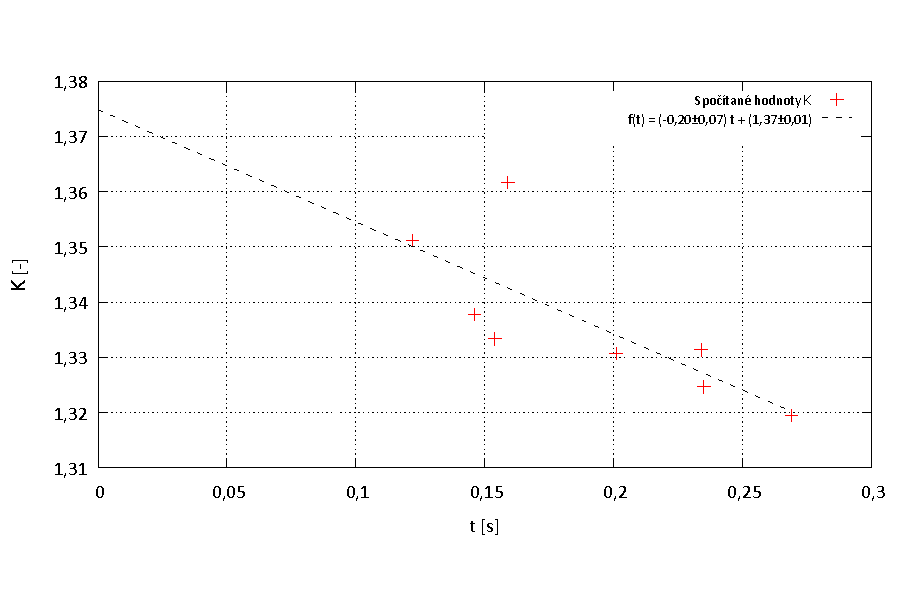
\includegraphics[width=\linewidth]{../gnuplot/data.pdf}
	    \vspace*{-1.5cm}
	    	\caption{Graf závislosti Poissonovy konstanty $\varkappa$ na době otevření ventilu $t$ a lineární extrapolace do nuly.}
			\label{fig:graf}
	\end{center}
	\end{figure}		

% Table generated by Excel2LaTeX from sheet 'List1'
\begin{table}[htbp]
\catcode`\-=12 % HAX na enable cline v českym bable
  \centering
    \begin{tabular}{|r|r|}
    \hline
    $n$ [-] & $T$ [s] \bigstrut\\
    \hline
    866   & 0,346 \bigstrut\\
    \hline
    871   & 0,344 \bigstrut\\
    \hline
    871   & 0,344 \bigstrut\\
    \hline
    881   & 0,341 \bigstrut\\
    \hline
    883   & 0,340 \bigstrut\\
    \hline
    885   & 0,339 \bigstrut\\
    \hline
    860   & 0,349 \bigstrut\\
    \hline
    868   & 0,346 \bigstrut\\
    \hline
    871   & 0,344 \bigstrut\\
    \hline
    871   & 0,344 \bigstrut\\
    \hline
    873   & 0,344 \bigstrut\\
    \hline
    874   & 0,343 \bigstrut\\
    \hline
    871   & 0,344 \bigstrut\\
    \hline
    877   & 0,342 \bigstrut\\
    \hline
    878   & 0,342 \bigstrut\\
    \hline\hline
    $\overline{T}$ [s] & 0,3435 \bigstrut\\
    \hline
    $\sigma_{\overline{T}}$ [s] & 0,0007 \bigstrut\\
    \hline
    \end{tabular}%

\caption{ Naměřené a vypočítané hodnoty při měření Poissonovy konstanty metodou kmitajícího pístku: $n$ je počet kmitů pístku za pět minut, $T$ z toho spočítané periody kmitů.  $\overline{T}$ je pak jejich aritmetický průměr se svojí chybou $\sigma_{\overline{T}}$ (\ref{eq:chyba_aritmetickeho_prumeru}).  } \label{tab:pistek}%
\end{table}%

%
%\clearpage
%\subsection{Schémata}
%
%\clearpage
	
% --- Konec dokumentu --------------------------------------------------


\end{document}

